% Final paper -- Artificial Intelligence and Economic Modeling (UP 2026-II)
%
% Body: 8 to 20 pages in THIS format (11pt, 1-inch margins, single column).
% Do not change the geometry or the font size to fit the limit.
% References and appendices do not count towards the limit.
\documentclass[11pt]{article}
\usepackage[utf8]{inputenc}
\usepackage[T1]{fontenc}
\usepackage[margin=1in]{geometry}
\usepackage{amsmath,amssymb,amsthm}
\usepackage{booktabs}
\usepackage{graphicx}
\usepackage{xcolor}
\usepackage[round]{natbib}
\usepackage[colorlinks=true,allcolors=blue!50!black]{hyperref}

\newtheorem{proposition}{Proposition}
\newtheorem{lemma}{Lemma}
\newtheorem{corollary}{Corollary}
\theoremstyle{definition}
\newtheorem{assumption}{Assumption}
\newtheorem{definition}{Definition}

% Every \replace box is an instruction to you, not text for the reader.
% A submitted paper has none left: delete the macro to be sure.
\newcommand{\replace}[1]{\par\smallskip\noindent
  \fcolorbox{orange!80!black}{yellow!12}{\parbox{\dimexpr\linewidth-2\fboxsep-2\fboxrule}{%
  \small\textbf{Replace.} #1}}\par\smallskip}

\title{Your Title: State the Result, Not the Topic}
\author{Your Name\thanks{Universidad del Pac\'ifico. Repository:
  \url{https://github.com/your-user/ai-project}. Track A (extension of a course
  paper) or Track B (thesis model): say which.}}
\date{\today}

\begin{document}
\maketitle

\begin{abstract}
\noindent\replace{One paragraph, at most 150 words: the question, the model in
one sentence, the main result \emph{with its condition}, and what the Lean
formalization does and does not certify.}
\end{abstract}

\section{Introduction}
\replace{The question, why it matters, and your answer. State the main result
in words in the first page. Say which paper you extend and which assumption you
relax (Track A), or which thesis model you formulate (Track B). End with what
is new relative to the closest paper. The toy model below only shows the
mechanics of this template; none of it is yours to keep.}

\section{Related literature}
\replace{Two or three paragraphs. Position the paper against the closest
work, cite the exact result you depart from (proposition and page), and check
the editorial status of every preprint you cite.}

The task-based view of automation follows \citet{acemoglu2018race}; the
decision-theoretic view of AI assistance follows \citet{agrawal2025bicycles}.

\section{Model}\label{sec:model}
\replace{Primitives, timing, information, and the agent's problem written
formally: what is maximised, over which variable, subject to which
constraints. Number every assumption; a result may only use numbered
assumptions.}

A worker chooses effort $e \ge 0$. Output is $a e$, where $a$ is productivity
with AI assistance, and effort costs $\tfrac{c}{2}e^{2}$.

\begin{assumption}\label{ass:params}
$a > 0$ and $c > 0$.
\end{assumption}

The worker solves
\begin{equation}\label{eq:problem}
  \max_{e \ge 0}\; a e - \frac{c}{2}\, e^{2}.
\end{equation}

\section{Results}\label{sec:results}
\replace{Every proposition with \emph{all} its conditions and a complete
proof. A proof may be moved to Appendix~\ref{app:proofs}, but the statement and
the idea of the proof stay here.}

\begin{proposition}\label{prop:effort}
Under Assumption~\ref{ass:params}, problem~\eqref{eq:problem} has the unique
solution $e^{*} = a/c$, and $\partial e^{*}/\partial a = 1/c > 0$.
\end{proposition}

\begin{proof}
The objective is twice differentiable with second derivative $-c < 0$, so it is
strictly concave and has at most one maximiser. The first-order condition
$a - c e = 0$ gives $e = a/c$, which is positive under
Assumption~\ref{ass:params}, so the constraint $e \ge 0$ does not bind and
$e^{*} = a/c$. Differentiating, $\partial e^{*}/\partial a = 1/c > 0$.
\end{proof}

\section{Simulations}\label{sec:sim}
\replace{A symbolic or numerical check of every result (SymPy, Monte Carlo, or
both), produced by the scripts in \texttt{code/}. Say what the simulation can
and cannot show: it checks a derivation on a grid, it does not prove it.}

Figure~\ref{fig:check} compares the closed form of
Proposition~\ref{prop:effort} with a grid search over $e$. The largest
absolute gap is reported by \texttt{code/verify.py}, which fails if it exceeds
the grid resolution.

\begin{figure}[ht]
  \centering
  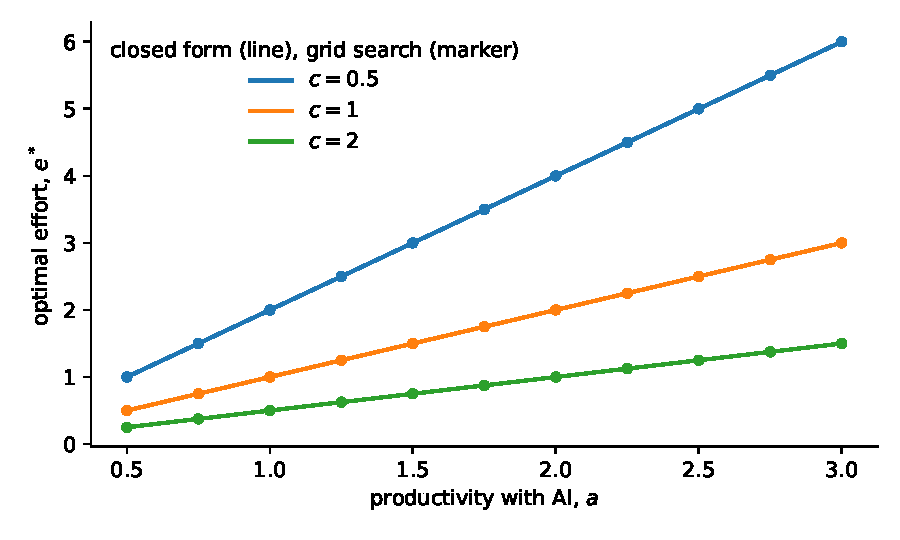
\includegraphics[width=.72\linewidth]{../code/figures/effort_check.pdf}
  \caption{Optimal effort: closed form (lines) and grid search (markers).
  Source: \texttt{code/verify.py}.}
  \label{fig:check}
\end{figure}

\section{Discussion and limitations}
\replace{What the result depends on, which assumption does the work, and what
you could not prove. A stated limitation is worth more than a hidden one.}

\section{Conclusion}
\replace{One paragraph. No new results.}

\bibliographystyle{plainnat}
\bibliography{references}

\appendix

\section{Omitted proofs}\label{app:proofs}
\replace{Proofs and derivations moved out of the body. The handwritten,
step-by-step version of every derivation lives in \texttt{hand/}.}

\section{Lean formalization}\label{app:lean}
\replace{One row per numbered result of the paper. ``Status'' is one of:
\emph{proved} (no \texttt{sorry}, no added hypothesis), \emph{proved under an
added hypothesis} (state it), or \emph{open} (state the exact blocker). Report
the paper commit that was formalized and the output of
\texttt{paper\_contribution.py check <Folder> --fast}.}

\begin{center}
\begin{tabular}{llll}
\toprule
Paper & Lean declaration & File in \texttt{lean/} & Status \\
\midrule
Proposition~\ref{prop:effort} & \texttt{<Folder>.prop\_effort} &
  \texttt{MainTheorems.lean} & \emph{example row} \\
\bottomrule
\end{tabular}
\end{center}

\section{AI collaboration log}\label{app:ai}
\replace{For each relevant contribution of a language model: what it claimed,
your verdict (correct, incorrect, or not verifiable) with the reason, and how
you checked it. The raw prompts and answers are in \texttt{prompts.md}.}

\begin{center}
\begin{tabular}{p{.30\linewidth}p{.22\linewidth}p{.36\linewidth}}
\toprule
Claim by the model & Verdict & How it was checked \\
\midrule
\emph{example:} ``$e^{*}=a/c$ for any $a$'' & Incorrect as stated &
  Fails for $a \le 0$: the corner $e^{*}=0$ binds. Hand derivation, p.~1. \\
\bottomrule
\end{tabular}
\end{center}

\end{document}
